\documentclass[]{elsarticle} %review=doublespace preprint=single 5p=2 column
%%% Begin My package additions %%%%%%%%%%%%%%%%%%%
\usepackage[hyphens]{url}

  \journal{An awesome journal} % Sets Journal name


\usepackage{lineno} % add
\providecommand{\tightlist}{%
  \setlength{\itemsep}{0pt}\setlength{\parskip}{0pt}}

\bibliographystyle{elsarticle-harv}
\biboptions{sort&compress} % For natbib
\usepackage{graphicx}
\usepackage{booktabs} % book-quality tables
%%%%%%%%%%%%%%%% end my additions to header

\usepackage[T1]{fontenc}
\usepackage{lmodern}
\usepackage{amssymb,amsmath}
\usepackage{ifxetex,ifluatex}
\usepackage{fixltx2e} % provides \textsubscript
% use upquote if available, for straight quotes in verbatim environments
\IfFileExists{upquote.sty}{\usepackage{upquote}}{}
\ifnum 0\ifxetex 1\fi\ifluatex 1\fi=0 % if pdftex
  \usepackage[utf8]{inputenc}
\else % if luatex or xelatex
  \usepackage{fontspec}
  \ifxetex
    \usepackage{xltxtra,xunicode}
  \fi
  \defaultfontfeatures{Mapping=tex-text,Scale=MatchLowercase}
  \newcommand{\euro}{€}
\fi
% use microtype if available
\IfFileExists{microtype.sty}{\usepackage{microtype}}{}
\usepackage{graphicx}
% We will generate all images so they have a width \maxwidth. This means
% that they will get their normal width if they fit onto the page, but
% are scaled down if they would overflow the margins.
\makeatletter
\def\maxwidth{\ifdim\Gin@nat@width>\linewidth\linewidth
\else\Gin@nat@width\fi}
\makeatother
\let\Oldincludegraphics\includegraphics
\renewcommand{\includegraphics}[1]{\Oldincludegraphics[width=\maxwidth]{#1}}
\ifxetex
  \usepackage[setpagesize=false, % page size defined by xetex
              unicode=false, % unicode breaks when used with xetex
              xetex]{hyperref}
\else
  \usepackage[unicode=true]{hyperref}
\fi
\hypersetup{breaklinks=true,
            bookmarks=true,
            pdfauthor={},
            pdftitle={Amazonian forests functional resistance to a selective logging disturbance},
            colorlinks=false,
            urlcolor=blue,
            linkcolor=magenta,
            pdfborder={0 0 0}}
\urlstyle{same}  % don't use monospace font for urls

\setcounter{secnumdepth}{0}
% Pandoc toggle for numbering sections (defaults to be off)
\setcounter{secnumdepth}{0}
% Pandoc header



\begin{document}
\begin{frontmatter}

  \title{Amazonian forests functional resistance to a selective logging
disturbance}
    \author[1]{Camille Piponiot\corref{c1}}
   \ead{camille.piponiot@gmail.com} 
   \cortext[c1]{Corresponding Author}
    \author[]{TmFO authors}
  
  
    \author[1, 2]{Bruno Hérault}
   \ead{bruno.herault@cirad.fr} 
  
      \address[1]{Cirad, UR Forets et Societes, Montferrier-sur-Lez, France}
    \address[2]{INPHB, Yamoussoukro, Cote d'Ivoire}
  
  \begin{abstract}
  This is the abstract.
  
  It consists of two paragraphs.
  \end{abstract}
  
 \end{frontmatter}

\section{Introduction}\label{introduction}

importance of tropical forests: ecosystem services (carbon, biodiversity
conservation)

but large uncertainties on their future: rapid changes in climatic
conditions and land use \(\rightarrow\) increasing frequency and
intensity of disturbances

one widespread disturbance = selective logging (xxx Mha/yr). XXx\% of
tropical forests have been logged at least once -\textgreater{} future
of tropical forests. Logging in the tropics usually consists in the
selective harvests of a few commercial species: maintains most of the
forest cover but infrastructure (roads and skid trails) and tree felling
can have large impacts on the forest.

disturbances such as selective logging can affect the composition and
dynamics of tropical forests: change the global functioning of the
ecosystem. // forest recovery after a disturbance -\textgreater{} carbon
stocks (Piponiot et al. 2016), tree size distribution {[}xx{]}, species
composition (Avila et al. 2015), biodiversity {[}xx{]}

notion of resilience: measure of how well an ecosystem can cope with
disturbances and return to its original (pre-disturbance) state. 2
components = change in state (or resistance to a disturbance) + return
time (Hodgson, McDonald, and Hosken 2015). {[}introduce our conceptual
framework, disturbance intensity{]}

functional traits = xxx (definition). characterisation of ecosystem
functioning \(\rightarrow\) importance to understand how they are
affected by disturbances. functional strategies and tradeoffs in
forests: leaf and wood economic spectrum, stature, and seed dispersal
strategy; explain most of the variation (Baraloto et al. 2012,
Costa-Saura et al. (2019)). selective logging disturbance
-\textgreater{} canopy openings, light -\textgreater{} colonisation by
small-seed light-wood species (Poorter and Rose 2005,) -\textgreater{}
changes in functional composition (Carreño-Rocabado et al. 2012).

environmental control: soil, climate, disturbance history
-\textgreater{} affects functional composition (Costa-Saura et al. 2019)
and response to disturbance. =\textgreater{} spatial variation. example:
Amazonia, the largest tropical forest biome (50\% of all tropical
rainforest area) -\textgreater{} 2 large scale gradients that control
the dynamics of old-growth forests: dryness gradient (NW-SE) (Davidson
et al. 2012) that constraints vegetation growth, and a tree mortality
gradient (SW-NE) (Johnson et al. 2016) due to lower soil stability (C.
a. Quesada et al. 2012) and higher frequency of windstorms
(Espírito-Santo et al. 2014) in the southwestern part of Amazonia.

Here we assess the resistance of 4 functional traits (namely wood
density, seed mass, specific leaf area and maximum tree diameter) to
selective logging in Amazonia. We calibrate an original Bayesian
hierarchical model with data from xxx permanent forest plots from 15
long-term experimental sites. Our research questions are: (i) how are
functional traits affected by disturbances in

\section{Methods}\label{methods}

\subsection{Study sites}\label{study-sites}

TmFO sites description

\begin{itemize}
\tightlist
\item
  environmental covariates: table? maps in SM?
\end{itemize}

\subsection{Functional trait data
compilation}\label{functional-trait-data-compilation}

grouping plots xxx (cf piponiot2019)

Traits chosen:

\begin{itemize}
\item
  \(DBH95\): DBH 95th percentile (per species) as a proxy of the stature
\item
  \(logSeedMass\): median seed mass (log-transformed) as a proxy of the
  dispersal strategy
\item
  \(SLA\): median specific leaf area, as a proxy of the assimilation
  strategy and leaf economic spectrum
\item
  \(WD\): median wood density, as a proxy of growth rate and mechanical
  support
\end{itemize}

retrieved from xxx and estimated for each individual: by species or
genus or plot mean (see explanation package BIOMASS)

Selective logging typically targets big trees (DBH \(\geq\)
40\textasciitilde{}cm) belonging to a small group of species with
commercial value.Those species usually have particular functional trait
values, such as large maximum diameters and high wood density {[}xx{]}.
The functional composition of the biggest trees is thus artificially
modified because of the selectivity of harvests. Because we are more
interested in the indirect effects of selective logging on the
functional composition, i.e.~the functional changes induced by tree
felling and canopy openings, we excluded trees with DBH \textgreater{}
35 cm from the analysis.

Mean weighted trait: (weighted with biomass)

\begin{equation}  
MWT_{k,c,p,s} = \frac{\sum_{i \in I_{c,p,s}}(T_{k,i}\cdot agb_i)}{\sum_{i \in I_{c,p,s}}(agb_i)}
\end{equation}

with \(T_{k,i}\) the value of trait \(k\) (either \(DBH95\),
\(logSeedMass\), \(SLA\), or \(WD\)) for individual tree \(i\),
\(agb_i\) the aboveground biomass of individual tree \(i\), and
\(I_{c,p,s}\) all live trees with DBH \(\geq\) 10\textasciitilde{}cm and
\(\leq\) 35\textasciitilde{}cm at census \(c\) in plot \(p\) in site
\(s\).

The aboveground biomass of each individual was estimated using the
package BIOMASS ({\textbf{???}}) (details xx).

\subsection{Conceptual model}\label{conceptual-model}

For each trait \(k\), the mean biomass-weighted trait of small trees
(MWT) trajectory at census \(c\) in plot \(p\) in site \(s\) was
modelled as:

\begin{equation}  
dMWT_{k,c,p,s} = \frac{MWT_{k,c,p,s} - MWT0_{k,p,s}}{T0_{k,p,s}} \sim \mathcal{N}\left( \mu_{k,c,p,s}\text{ , } \left(\frac{\sigma_k}{size_p}\right)^2\right)
\end{equation}

with

\begin{equation}  
\mu_{k,c,p,s} = \Delta_{k,p,s} \cdot \left( \frac{t_c}{tmax_{k,p,s}} \cdot exp\left(1-\frac{t_c}{tmax_{k,p,s}}\right) \right)^{\theta_{k,p,s}}
\end{equation}

\begin{itemize}
\item
  \(c\) the census, and \(t_c\) the time since logging (in years) at
  census \(c\),
\item
  \(T0_{k,p,s}\) the pre-logging trait value of the community in plot
  \(p\) in site \(s\).
\item
  \(\Delta_{k,p,s}\) is the maximum value (relative to the final value)
  of the hump that follows logging and the creation of logging gaps.
  \(\Delta_{k,p,s} \sim \mathcal{N} (\mu_{\Delta ks}, \sigma_{\Delta}^2)\),
  with \(\mu_{\Delta ks}\) and \(\sigma_{\Delta}\) are respectively the
  mean and standard deviation of \(\Delta\) for trait \(k\) in site
  \(s\).
\item
  \(tmax_{k,p,s}\) is the time when the maximum value of the hump is
  reached. \(tmax_{k,p} = 0\) for control plots and in logged plots
  \(tmax_{k,p} \sim \mathcal{N} (\mu m_{ k}, \sigma m^2)\) where
  \(\mu m_{k}\) and \(\sigma m\) are respectively the mean and standard
  deviation of \(tmax\) for trait \(k\).
\item
  \(\theta_k\) is a shape parameter that controls the width of the hump;
  when it increases, the hump is narrower.
\item
  \(size_p\) is the size of plot \(p\)
\end{itemize}

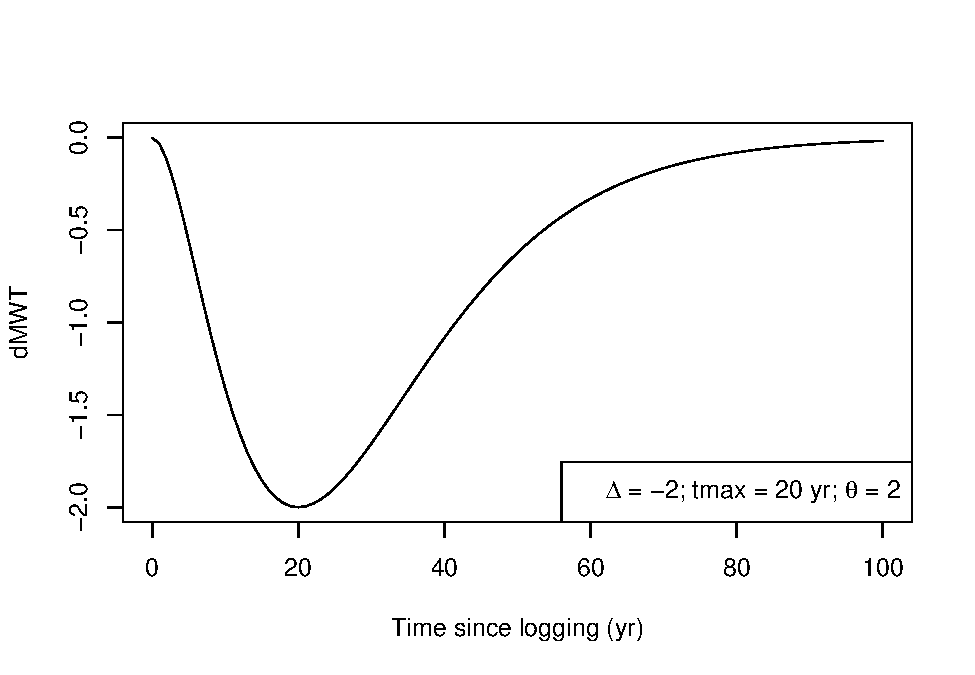
\includegraphics{rticle_tmfo_functional_files/figure-latex/unnamed-chunk-1-1.pdf}

\(\Delta_{k,p,s}\) is the maximum change of trait \(k\) after the
disturbance: its absolute value is expected to increase with disturbance
intensity. We thus modelled it as:

\begin{equation} 
\Delta_{k,p,s} = loss_p \cdot (\lambda_{0,k} + \sum \lambda_{m,k} Cov_{m,s}) 
\end{equation}

\(loss_p\) is the relative aboveground biomass loss after logging in
plot \(p\), as a proxy of the disturbance intensity; it is estimated as
the difference between the pre-logging aboveground biomass and the
minimum biomass in the first 4 years after logging, divided by the
pre-logging aboveground biomass. \(Cov_{m,s}\) is the value of covariate
\(m\) (either the mortality rate or the climatic water deficit) in site
\(s\).

\subsection{Model calibration}\label{model-calibration}

\section{Results}\label{results}

\subsection{Predictions fitness}\label{predictions-fitness}

\subsection{Traits variation and resistance to
logging}\label{traits-variation-and-resistance-to-logging}

\subsection{Spatial variation}\label{spatial-variation}

\section{Discussion}\label{discussion}

\section*{References}\label{references}
\addcontentsline{toc}{section}{References}

\hypertarget{refs}{}
\hypertarget{ref-DeAvila2015}{}
Avila, Angela Luciana de, Ademir Roberto Ruschel, João Olegário Pereira
de Carvalho, Lucas Mazzei, José Natalino Macedo Silva, José do Carmo
Lopes, Maristela Machado Araujo, Carsten F. Dormann, and Jürgen Bauhus.
2015. ``Medium-term dynamics of tree species composition in response to
silvicultural intervention intensities in a tropical rain forest.''
\emph{Biological Conservation} 191. Elsevier B.V.: 577--86.
doi:\href{https://doi.org/10.1016/j.biocon.2015.08.004}{10.1016/j.biocon.2015.08.004}.

\hypertarget{ref-Baraloto2012a}{}
Baraloto, Christopher, Olivier J Hardy, C E Timothy Paine, Kyle G
Dexter, Corinne Cruaud, Luke T Dunning, Mailyn-Adriana Gonzalez, et al.
2012. ``Using functional traits and phylogenetic trees to examine the
assembly of tropical tree communities.'' \emph{Journal of Ecology} 100
(3): 690--701.
doi:\href{https://doi.org/10.1111/j.1365-2745.2012.01966.x}{10.1111/j.1365-2745.2012.01966.x}.

\hypertarget{ref-Carreno-Rocabado2012}{}
Carreño-Rocabado, Geovana, Marielos Peña-Claros, Frans Bongers, Alfredo
Alarcón, Juan Carlos Licona, and Lourens Poorter. 2012. ``Effects of
disturbance intensity on species and functional diversity in a tropical
forest.'' \emph{Journal of Ecology} 100 (6): 1453--63.
doi:\href{https://doi.org/10.1111/j.1365-2745.2012.02015.x}{10.1111/j.1365-2745.2012.02015.x}.

\hypertarget{ref-Costa-Saura2019}{}
Costa-Saura, José M., Antonio Trabucco, Donatella Spano, and Simone
Mereu. 2019. ``A height-wood-seed axis which is preserved across
climatic regions explains tree dominance in European forest
communities.'' \emph{Plant Ecology} 0123456789.
doi:\href{https://doi.org/10.1007/s11258-019-00928-x}{10.1007/s11258-019-00928-x}.

\hypertarget{ref-Davidson2012}{}
Davidson, Eric a., Alessandro C. de Araújo, Paulo Artaxo, Jennifer K.
Balch, I. Foster Brown, Mercedes M. C. Bustamante, Michael T. Coe, et
al. 2012. ``The Amazon basin in transition.'' \emph{Nature} 481 (7381):
321--28.
doi:\href{https://doi.org/10.1038/nature10717}{10.1038/nature10717}.

\hypertarget{ref-Espirito-Santo2014}{}
Espírito-Santo, Fernando D.B., Manuel Gloor, Michael Keller, Yadvinder
Malhi, Sassan Saatchi, Bruce Nelson, Raimundo C Oliveira Junior, et al.
2014. ``Size and frequency of natural forest disturbances and the Amazon
forest carbon balance.'' \emph{Nature Communications} 5 (March): 3434.
doi:\href{https://doi.org/10.1038/ncomms4434}{10.1038/ncomms4434}.

\hypertarget{ref-Hodgson2015}{}
Hodgson, Dave, Jenni L. McDonald, and David J. Hosken. 2015. ``What do
you mean, 'resilient'?'' \emph{Trends in Ecology and Evolution} 30 (9).
Elsevier Ltd: 503--6.
doi:\href{https://doi.org/10.1016/j.tree.2015.06.010}{10.1016/j.tree.2015.06.010}.

\hypertarget{ref-Johnson2016}{}
Johnson, Michelle O., David Galbraith, Manuel Gloor, Hannes De
Deurwaerder, Matthieu Guimberteau, Anja Rammig, Kirsten Thonicke, et al.
2016. ``Variation in stem mortality rates determines patterns of
above-ground biomass in Amazonian forests: implications for dynamic
global vegetation models.'' \emph{Global Change Biology} 22 (12):
3996--4013.
doi:\href{https://doi.org/10.1111/gcb.13315}{10.1111/gcb.13315}.

\hypertarget{ref-Piponiot2016a}{}
Piponiot, Camille, Plinio Sist, Lucas Mazzei, Marielos Peña-Claros,
Francis E Putz, Ervan Rutishauser, Alexander Shenkin, et al. 2016.
``Carbon recovery dynamics following disturbance by selective logging in
Amazonian forests.'' \emph{eLife} 5 (C).
doi:\href{https://doi.org/10.7554/eLife.21394}{10.7554/eLife.21394}.

\hypertarget{ref-Poorter2005a}{}
Poorter, Lourens, and Simmoné A. Rose. 2005. ``Light-dependent changes
in the relationship between seed mass and seedling traits: A
meta-analysis for rain forest tree species.'' \emph{Oecologia} 142 (3):
378--87.
doi:\href{https://doi.org/10.1007/s00442-004-1732-y}{10.1007/s00442-004-1732-y}.

\hypertarget{ref-Quesada2012}{}
Quesada, C. a., O. L. Phillips, M. Schwarz, C. I. Czimczik, T. R. Baker,
S. Patiño, N. M. Fyllas, et al. 2012. ``Basin-wide variations in Amazon
forest structure and function are mediated by both soils and climate.''
\emph{Biogeosciences} 9 (6): 2203--46.
doi:\href{https://doi.org/10.5194/bg-9-2203-2012}{10.5194/bg-9-2203-2012}.

\end{document}


